\documentclass[12pt,a4paper]{article}
\usepackage[utf8]{inputenc}
\usepackage[english]{babel}
\usepackage[T1]{fontenc}
\usepackage{amsmath}
\usepackage{amsfonts}
\usepackage{amssymb}
\usepackage{graphicx}
\usepackage{siunitx}
\usepackage{float}
\usepackage[left=2cm,right=2cm,top=2cm,bottom=2cm]{geometry}
\author{Gerald}

\begin{document}
\sisetup{separate-uncertainty = true}
	\setlength{\parindent}{0pt} 
	\begin{center}
		{\LARGE Experiment protocol}\\
		\begin{large}
			for the solid state lab course\\[0.4cm]
			at RWTH Aachen\\
			II. Physikalisches Institut A\\[5.5cm]
			\Large\textbf{\textsl{Superconductivity and SQUID}}\\[5.5cm]
			\normalsize\textit{authored\\by}\\[0.4cm]
			\large{Moritz Berger (355244)\\Gerald Kolter (355005)}\\[2cm]
			\large \textbf{Summer term 2019}
		\end{large}
	\end{center}
	\newpage
	
	\tableofcontents
	\newpage

\section{Introduction}
Superconducting Quantum Information Devices ("SQUIDS") are very sensitive sensors for magnetic flux. A SQUID consists of a ring shaped superconductor with two contacts and each one Josephson junction on each path between the contacts. A Josephson junction is a small insulator between two superconductors. Electrons can tunnel through the insulator as Cooper pairs. \\
The resolution of the measured magnetic flux is in the order of the so called fluxonium or flux quantum:
\begin{equation*}
\Phi _0 = \dfrac{h}{2e} = 2 \times 10^{-15}\si{Wb}
\end{equation*}


\section{Goal of the Experiment}
The goal of the experiment is to first determine the critical temperature of the superconducting material $T_C$. \\
With the SQUID cooled down to the superconducting regime one measures the voltage-current characteristic. From this one can determine the critical current $I_C$, the resistance in the normal conducting state $R_N$ and the characteristic voltage $V_C$. \\
Next one measures the voltage-magnetic flux characteristic. From this one determines the SQUID parameter $b_L$ given by:
\begin{equation}
b_L = 2 \cdot I_C \cdot \dfrac{L}{\Phi _0}
\end{equation}
And with that the magnetic flux quantum $\Phi _0$. \\
With bringing different metallic objects in the vicinity of the SQUID one can demonstrate the sensitivity of the SQUID to external magnetic fields. This is done with and without the metallic shielding of the SQUID.


\section{Setup}
The setup consits of a SQUID in a metallic tube, which shields external magnetic fields. This setup is called "Mr. SQUID" and selled by the company "Conductus". The SQUID is sinked in a dewar filled with liquid nitrogen to cool it down to the necessary temperatures. \\
The SQUID itself is build out of Yba$_2$Cu$_3$O$_{7-x}$ with $x \approx 0-0.2$. The temperature is measured with a Pt-100 resistor.


\section{Temperature Calibration}
\subsection{Measurement}
The temperature is measured with a Pt-100 resistor, which measures a resistance. For the calibration the resistance at room temperature, measured with a thermometer, and at the temperature of the liquid nitrogen. For this the SQUID including the resistor is sinked into the liquid nitrogen and the resistance is measured after it stabalized. In this area a linear dependence between the resistance and the temperature is assumed.

\subsection{Data}

\begin{figure} [H]
\centering
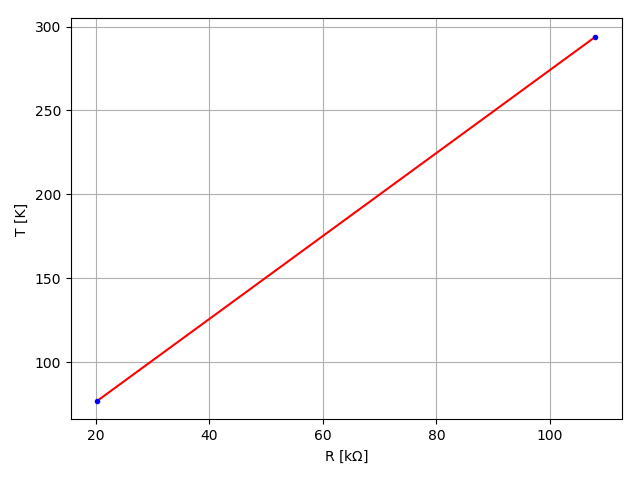
\includegraphics[scale=0.8]{Bilder/Temp_kalibration.PNG}
\caption{Temperature calibration for the Pt-100 resistor.}
\label{fig:Temp_kalibration}
\end{figure}

Fig. \ref{fig:Temp_kalibration} shows the calibration. The two points are the two measurements and the orange line is the linear calibration. 

\subsection{Results}

\begin{table} [H]
\centering
\begin{tabular}{|c|c|c|c|}
\hline 
$T_{room}$ [K] & $T_{LN_2}$ [K] & $R_{RT}$ [k$\Omega$] & $R_{LN_2}$ [k$\Omega$] \\ 
\hline 
294.65 $\pm$ $\frac{1}{\sqrt{12}}$ & 77 $\pm$ $\frac{1}{\sqrt{12}}$ & 107.9 $\pm$ $\frac{1}{\sqrt{12}}$ & 20.3 $\pm$ $\frac{1}{\sqrt{12}}$ \\ 
\hline 
\end{tabular} 
\caption{Measured values for the resistance at room temperature and the temperature of liquid nitrogen.}
\label{tab:Temp_Calib_data}
\end{table}

For a measured resistance from the Pt-100 resistor $R_{measured}$ one can calculate the temperature with:
\begin{equation*}
T = \dfrac{T_{room} - T_{LN_2}}{R_{RT} - R_{LN_2}} \cdot R_{measured} + T_{room} - \dfrac{T_{room} - T_{LN_2}}{R_{RT} - R_{LN_2}} \cdot R_{RT}
\end{equation*}
With $R_{RT}$ being the resistance measured at room temperature, $R_{LN_2}$ the resistance at the temperature of liquid nitrogen, $T_{room}$ the room temperature and $T_{LN_2}$ the temperature of liquid nitrogen. With assuming the same error on all resistance measurements $\sigma _R = \frac{\SI{1}{k \Omega}}{\sqrt{12}}$ and the same error on all temperature measurements $\sigma _T = \frac{\SI{1}{K}}{\sqrt{12}}$ the error propagation is straight forward.


\section{Temperature Dependence of the Resistance}
\subsection{Measurement}
The voltage in dependence of the current is measured while the sample is slowly cooled down. For that purpose the sample is moved down slowly in the dewar while not being in contact with with the liquid nitrogen.

\subsection{Data}

\begin{figure} [H]
\centering
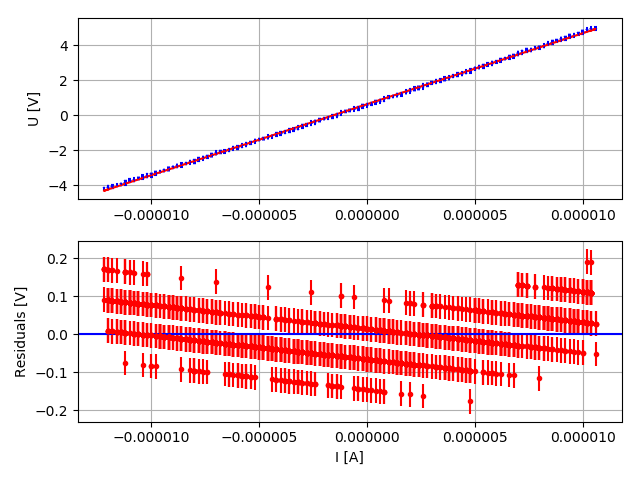
\includegraphics[scale=0.8]{Bilder/Critical_Temperature/Resistance_fit_13.PNG}
\caption{SQUID voltage in dependence of the current at \SI{237 \pm 2}{K}.}
\label{fig:Temp_Resistance_example}
\end{figure}

Fig. \ref{fig:Temp_Resistance_example} shows exemplary one of the measured curves for the SQUID voltage in dependence of the current at \SI{237 \pm 2}{K}. The slope yields the resistance of the SQUID at that point so its extracted with a linear fit, which is already done in the shown plot.

\subsection{Results}

\begin{figure} [H]
\centering
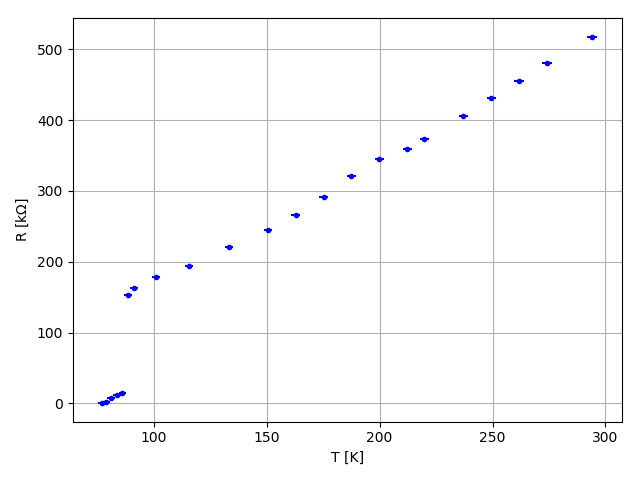
\includegraphics[scale=0.8]{Bilder/Critical_Temperature/Temp_Resistance.PNG}
\caption{SQUID resistance in dependence of the temperature.}
\label{fig:Temp_Resistance}
\end{figure}

Fig. \ref{fig:Temp_Resistance} shows the completed plot of the resistance vs. the temperature. As expected there is a big drop in the resistance at a certain temperature. \\
The critical temperature at which the resistance drops can be read off by taking the two points limiting the drop, i.e. the lowest point above and the highest below the drop. The critical temperature is estimated by the mean value of these two and the error by the difference devided by $\sqrt{12}$. This leads to the value:
\begin{equation*}
T_C = \SI{87.39 \pm 0.71}{K}
\end{equation*}


\section{U-I-Characteristic}
\subsection{Measurement}
With the sample sinked in the liquid nitrogen and after temperature stabilisation the voltage in dependence of the current is measured.

\subsection{Data}

\begin{figure} [H]
\centering
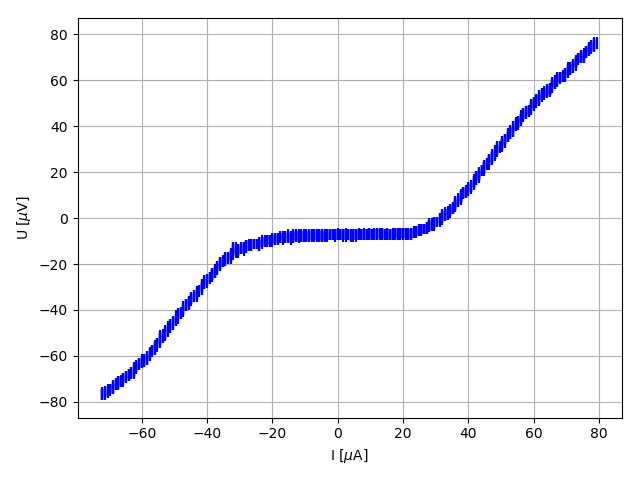
\includegraphics[scale=0.8]{Bilder/U_I_characteristic/characteristic.PNG}
\caption{U-I characteristic of the SQUID in the superconducting state.}
\label{fig:U-I-characteristic}
\end{figure}

Fig. \ref{fig:U-I-characteristic} shows the U-I characteristic of the SQUID in the superconducting state. As expected one can see a plateau around zero current. Outside from that one sees a linear dependence.

\subsection{Results}

\begin{figure} [H]
\centering
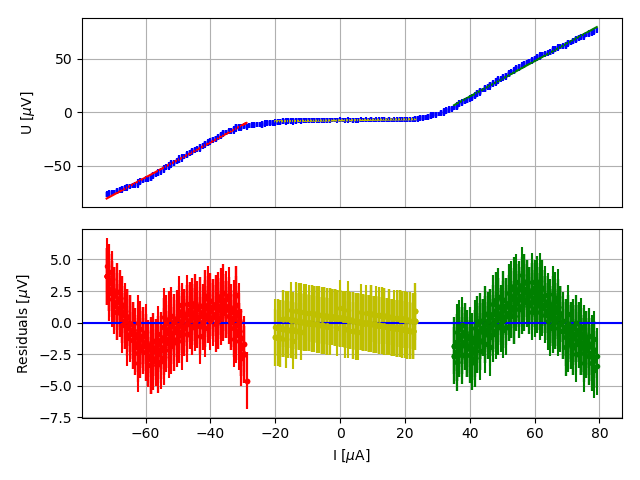
\includegraphics[scale=0.8]{Bilder/U_I_characteristic/fit_43.PNG}
\caption{U-I characteristic of the SQUID in the superconducting state.}
\label{fig:U-I-characteristic_fit}
\end{figure}




\section{Conclusion}






\end{document}